\documentclass[10pt,paper=letter]{scrartcl}
\usepackage[alttitle]{cjquines}

\begin{document}

\title{VCSMS PRIME}
\subtitle{Program for Inducing Mathematical Excellence}
\author{Session 11: Number Theory}
\date{October 20, 2017}

\maketitle
\setlength{\unitlength}{1in}
\begin{picture}(0,0)
  \put(5.5,0.5){\hbox{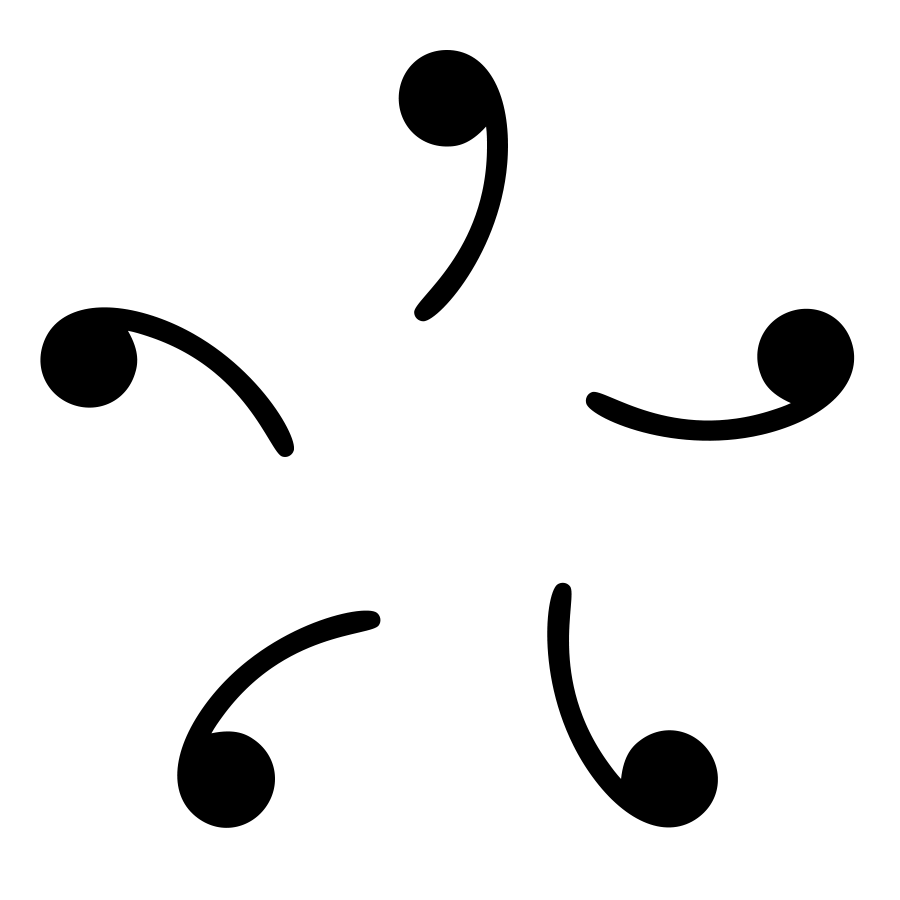
\includegraphics[width=0.9in]{logo.png}}}
\end{picture}
\vspace{-3.5em}

\subsubsection*{Lecture problems}

\begin{enumerate}
  \item For how many integers $4 < d < 2017$ is $441$ a perfect square in base $d$?
  \item (AI16) Let $N$ be a natural number whose base-$2016$ representation is $ABC$. Working now in base-$10$, what is the remainder when $N - (A + B + C + k)$ is divided by $2015$, for some $k \in \cbr{1, 2, \ldots, 2015}$?
  \item (AHSME 1993) Given $0 \leq x_0 < 1$ define $x_n$ for all positive integers $n$ to be $2x_{n-1}$ if $2x_{n-1} < 1$, or $2x_{n-1}-1$ otherwise. How many $x_0$ satisfy $x_0 = x_5$?
  \item (AIME 1986) The sequence $1, 3, 4, 9, 10, \ldots$ consists of the positive integers which are powers of three or sums of distinct powers of three. Find its hundredth term.
  \item (AIME 1985) Let $a_n = 100+n^2$ for all positive integral $n$. Find the maximum GCD of $a_n$ and $a_{n+1}$.
  \item (HMMT 2002) Find the greatest common divisor of all numbers of the form $2002^n + 2$ for $n \in \NN$.
  \item (QI11) When $2a$ is divided by $7$, the remainder is $5$. When $3b$ is divided by $7$, the remainder is also $5$. What is the remainder when $a+b$ is divided by $7$?
  \item (QII2) Suppose that $159aa72$ is a multiple of $2016$. What is the sum of its distinct prime divisors?
  \item (Canada 2003) Find the last three digits of $2003^{2002^{2001}}$.
  \item Factorize $89701$, $160401$ and $2^{18} + 1$.
  \item (QI8) How many positive divisors of $30^9$ are divisible by $400{,}000$?
  \item (AI12) Let $n = 2^{23}3^{17}$. How many factors of $n^2$ are less than $n$ but do not divide $n$?
  \item (QIII5) Let $s(n)$ be the number of terminal zeroes in the decimal representation of $n!$. How many positive integers less than $2017$ cannot be expressed in the form $n+s(n)$ for some positive integer $n$?
  \item How many ordered pairs of positive unit fractions have sum $\frac16$?
\end{enumerate}

\subsubsection*{Digits and bases}

\begin{itemize}
  \item Problem 1: All of them: $441_d = 4d^2 + 4d + 1 = (2d + 1)^2$ in base $10$.
  \item Problem 2: $N = C + 2016B + 2016^2A$ in base $10$. Then $N - (A + B + C + k) = 2015B + (2016^2-1)A - k$, but the first two terms are divisible by $2015$, so the remainder is $2015-k$.
  \item Problem 3: The doubling makes us consider binary. The sequence moves the decimal point to the right.
  \item Problem 4: Writing in ternary, these are the numbers that only have $0$ or $1$, so the terms are just binary.
\end{itemize}

\subsubsection*{Divisibility}

\begin{itemize}
  \item Note $a|b$ iff $(a, b) = a$. We have $(a, b) = (a-b, b)$. This gives the Euclidean algorithm.
  \item Problem 5: We have $(100 + n^2, 100 + (n+1)^2) = (100 + n^2, 2n + 1) = (200 + 2n^2, 2n + 1) = (200 - n, 2n + 1) = (400-2n, 2n+1) = (401, 2n+1)$.
  \item Problem 6: Equivalent to GCD of $2004$ and $2002^n - 2002 = 2002(2002^{n-1} -1)$. But it is well-known that $(a^n - 1, a^m - 1) = a^{\del{n, m}} - 1$.
\end{itemize}

\subsubsection*{Modulo}

\begin{itemize}
  \item The integers modulo a prime form a field. Thus we have arithmetic. For composite moduli, CRT. From most to least common, know how to solve linear systems, Fermat's Little, Euler Totient, Wilson, Lucas.
  \item Problem 7: $2a \equiv 5 \pmod 7$ implies $a \equiv 5\cdot2^{-1} \pmod 7$, but the inverse of $2$ is $4$ (trial-and-error, or $2x+7y=1$.), so $a \equiv 5\cdot4 \equiv 6 \pmod 7$. Similarly $b \equiv 4 \pmod 7$ and $a+b \equiv 3 \pmod 7$.
  \item Problem 8: $159aa72 \equiv 1590072 + 1100a \equiv 1464 + 1100a \equiv 0 \pmod{2016}$. Not hard to find $a$.
  \item Problem 9: Split into mod $8$ and mod $125$. Binary exponentiation for $3^{52}$ mod $125$.
\end{itemize}

\subsubsection*{Factorization}

\begin{itemize}
  \item Usually involves clever algebraic manipulation. If you end up with a number not in an obviously factorable way, always try to rewrite as difference of two squares.
  \item Problem 10: The first is $300^2 - 300 + 1 = (300 + 1)^2 - 900$. The second is $20^4 + 20^2 + 1 = (20^2 + 1)^2 - 20^2$. By Sophie--Germain, the last is $(1 - 2^5 + 2^{9})(1 + 2^5 + 2^{9})$.
\end{itemize}

\subsubsection*{Multiplicative number theory}

\begin{itemize}
  \item A function $f$ is multiplicative if $f(mn) = f(m)f(n)$ for all $(m, n) = 1$. Such a function is determined completely by powers of primes. Examples: $\tau(n)$, number of divisors; $\sigma(n)$, sum of divisors; $\phi(n)$, number of positive integers less than and relatively prime to $n$. 
  \item Problem 11: Answer is just $\tau(30^9/400{,}000)$.
  \item Problem 12: Each factor of $n^2$ has a pair that multiplies to $n^2$; one is smaller and one is larger than $n$, so $\frac12\del{\tau(n^2) - 1}$ is the number of factors less than $n$. These overcount the factors of $n$, subtract $\tau(n)$.
  \item ``Sum of divisors that are perfect squares'', ``that are even'', ``difference of divisors with odd sum of exponents and even sum of exponents'', ``product of divisors'' or ``sums of product of non-zero digits''.
\end{itemize}

\subsubsection*{Valuation}

\begin{itemize}
  \item $\nu_p(n)$ is the largest power of $p$ that divides $n$. Most important is $\nu_p(n!)$, which is given by de Polignac, $\floor{n/p} + \floor{n/p^2} + \cdots$. This allows us, for example, to compute the valuation for binomial coefficients. This is also equivalent to $(p-1)\nu_p(n!) = n - s_p(n)$ where $s_p(n)$ is the sum of the digits of $n$ in base $p$.
  \item Problem 13: The limiting factor of $10$ is $5$, so $s(n) = \nu_{5}{n!}$. The ``bumps'' happen at multiples of $5$. Alternatively, consider base $5$ and use the second version of de Polignac's.
\end{itemize}

\subsubsection*{Diophantine equations}

\begin{itemize}
  \item The building block is $ax + by = c$ for fixed $a, b, c$ and integers $x, y$. Bezout's: only need to solve the case $ax + by = (a,b)$. Then we only need to find one solution by using Euclidean algorithm or trial-and-error.
  \item Frobenius: if $(a, b) = 1$, for nonnegative $x, y$, the number of positive integers that can't be written as $ax+by$ is $\frac12(a-1)(b-1)$. Chicken McNugget: the largest that can't is $ab - a - b$.
  \item Finally, factorization, often SFFT, will take care of most other cases.
  \item Problem 14: Equation $\frac1a + \frac1b = \frac16$ is equiv to $6a + 6b = ab$, or $(6-a)(6-b)=36$. Casework on factors.
\end{itemize}

\end{document}
